\documentclass[12pt]{article}
\usepackage[utf8]{inputenc}
\usepackage{float}
\usepackage{amsmath}


\usepackage[hmargin=3cm,vmargin=6.0cm]{geometry}
\topmargin=-2cm
\addtolength{\textheight}{6.5cm}
\addtolength{\textwidth}{2.0cm}
\setlength{\oddsidemargin}{0.0cm}
\setlength{\evensidemargin}{0.0cm}
\usepackage{indentfirst}
\usepackage{amsfonts}

%
\usepackage{graphicx}
\usepackage[most]{tcolorbox}
\usepackage{multicol}
\usepackage{caption}

\newtcolorbox{mybox}[3][]
{
  colframe = #2!25,
  colback  = #2!10,
  coltitle = #2!20!black,  
  title    = {#3},
  #1,
}

%
\setlength{\parindent}{0pt}

% macros
\newcommand{\prob}[1]{\textbf{\textit{P}}\left\{#1\right\}}
\newcommand{\expc}[1]{\mathbf{E}\left(#1\right)}
\newcommand{\expcs}[1]{\mathbf{E}^2\left(#1\right)}
\newcommand{\var}[1]{\text{Var}\left( #1 \right)}

\newenvironment{formula}[1]{\begin{mybox}{cyan}{\textbf{#1}}}{\end{mybox}}

\begin{document}

% Bu ödevde emeği geçen herkesin tüm aile bireylerine sevgilerimi yolluyorum. Umuarım, bu ödevi verip bana çektirdiklerini çekmeden ölmezler, analarından babalarından, çocuklarından çıkar.

\section*{Student Information}

Name : Burak Metethan Tunçel\\

ID : 2468726\\

\section*{Answer 1}

\subsection*{a)}

\noindent \textit{They are \textbf{not independent}}. Independence formula for continuous variables is
\begin{equation*}
    f_{(X, Y)} (x, y) = f_X(x) f_Y(y)
\end{equation*}
So, we need to find equations for $f_X(x)$ and $f_Y(y)$.

\subsubsection*{Finding $f_X(x)$}

\begin{equation*}
    f_X(x) = \int_{-\infty}^{\infty} f_{(X, Y)} (x, y) dy
\end{equation*}

\noindent We can rewrite the function $f_{(X, Y)}(x, y)$ as follows,
\begin{equation*}
    f_{(X, Y)}(x, y) = \begin{cases}
        \dfrac{1}{\pi} &\textnormal{if $-\sqrt{1-x^2} \leq y \leq \sqrt{1-x^2}$}\\
        0 &\textnormal{otherwise}
    \end{cases}
\end{equation*}
One can say that for otherwise part, the integral is 0. For other part,
\begin{align*}
    f_X(x) &= \int_{-\sqrt{1-x^2}}^{\sqrt{1-x^2}} f_{(X, Y)}(x, y) dy\\
         &= \int_{-\sqrt{1-x^2}}^{\sqrt{1-x^2}} \frac{1}{\pi} dy\\
         &= \frac{2\sqrt{1-x^2}}{\pi} &-1 \leq x \leq 1
\end{align*}

\subsubsection*{Finding $f_Y(y)$}

\noindent Similarly, we can rewrite the function $f_{(X, Y)}(x, y)$ as follows,
\begin{equation*}
    f_{(X, Y)}(x, y) = \begin{cases}
        \dfrac{1}{\pi} &\textnormal{if $-\sqrt{1-y^2} \leq x \leq \sqrt{1-y^2}$}\\
        0 &\textnormal{otherwise}
    \end{cases}
\end{equation*}
From here,
\begin{align*}
    f_Y(y) &= \int_{-\sqrt{1-y^2}}^{\sqrt{1-y^2}} f_{(X, Y)}(x, y) dx\\
         &= \int_{-\sqrt{1-y^2}}^{\sqrt{1-y^2}} \frac{1}{\pi} dx\\
         &= \frac{2\sqrt{1-y^2}}{\pi} &-1 \leq y \leq 1
\end{align*}

\noindent In the end, we have
\begin{align*}
    f_X(x) &= \begin{cases}
                \dfrac{2\sqrt{1-x^2}}{\pi} &-1 \leq x \leq 1\\
                0 &\textnormal{otherwise}
            \end{cases}\\
    f_Y(y) &= \begin{cases}
                \dfrac{2\sqrt{1-y^2}}{\pi} &-1 \leq y \leq 1\\
                0 &\textnormal{otherwise}
            \end{cases}
\end{align*}

\noindent So back to formula
\begin{equation*}
    \left[ f_{(X, Y)}(x, y) = \begin{cases}
        \dfrac{1}{\pi} &x^2 + y^2 \leq 1\\
        0 &\textnormal{otherwise}
    \end{cases} \right]\
    \
    \
    \neq \left[ f_X(x) f_Y(y) = \begin{cases}
        \dfrac{2\sqrt{1-x^2}}{\pi} \cdot \dfrac{2\sqrt{1-y^2}}{\pi} &-1 \leq x \leq 1, -1 \leq y \leq 1\\
        0 &\textnormal{otherwise}
    \end{cases} \right]
\end{equation*}

\noindent Also, we can show that they are dependent if we find at least 1 pair that violates the independecy equation. Let $x = y = \dfrac{\sqrt{3}}{2}$, then
\begin{equation*}
    f_{(X, Y)}\left(\dfrac{\sqrt{3}}{2}, \dfrac{\sqrt{3}}{2}\right) = \frac{1}{\pi} \neq \frac{1}{\pi^2} = f_X\left(\dfrac{\sqrt{3}}{2}\right) f_Y\left(\dfrac{\sqrt{3}}{2}\right)
\end{equation*}

\subsection*{b)}

From part a,
\begin{align*}
    f_X(x) &= \begin{cases}
                \dfrac{2\sqrt{1-x^2}}{\pi} &-1 \leq x \leq 1\\
                0 &\textnormal{otherwise}
            \end{cases}\\
    f_Y(y) &= \begin{cases}
                \dfrac{2\sqrt{1-y^2}}{\pi} &-1 \leq y \leq 1\\
                0 &\textnormal{otherwise}
            \end{cases}
\end{align*}

\subsection*{c)}

Since our pdf is piecewise, we need the calculate each piece one by one,
\begin{align*}
    \expc{X} = \mu &= \int_{-\infty}^{\infty} x f_X(x) dx\\
                        &= \int_{-\infty}^{-1} x f_X(x) dx + \int_{-1}^{1} x f_X(x) dx + \int_{1}^{\infty} x f_X(x) dx\\
                        &= \int_{-\infty}^{-1} x 0 dx + \int_{-1}^{1} x \dfrac{2\sqrt{1-x^2}}{\pi} dx + \int_{1}^{\infty} x 0 dx\\
                        &= \int_{-\infty}^{-1} 0 dx + \int_{-1}^{1} x \dfrac{2\sqrt{1-x^2}}{\pi} dx + \int_{1}^{\infty} 0 dx\\
                        &= 0 + \left[ -\frac{2}{\pi} \cdot \frac{1}{3} \left( 1 - x^2 \right)^{\frac{3}{2}} \right]\Biggl|_{-1}^{1} + 0\\
                        &= \left[ -\frac{2}{\pi} \cdot \frac{1}{3} \left( 1 - 1^2 \right)^{\frac{3}{2}} \right] - \left[ -\frac{2}{\pi} \cdot \frac{1}{3} \left( 1 - (-1)^2 \right)^{\frac{3}{2}} \right]\\
                        &= 0 - 0 = 0
\end{align*}

\subsection*{d)}

Since our pdf is piecewise, we need the calculate each piece one by one,
\begin{align*}
    \var{X} &= \expc{X - \mu^2}^2\\
            &= \int_{-\infty}^{\infty} \left( x - \mu \right)^2 f_X(x) dx\ \ \ \ \ (\mu = 0)\\
            &= \int_{-\infty}^{\infty} x^2 f_X(x) dx\\
            &= \int_{-\infty}^{-1} x^2 f_X(x) dx + \int_{-1}^{1} x^2 f_X(x) dx + \int_{1}^{\infty} x^2 f_X(x) dx\\
            &= 0 + \int_{-1}^{1} x^2 \dfrac{2\sqrt{1-x^2}}{\pi} dx + 0\\
            &= \left[ \frac{1}{16\pi} \left( 4 \arcsin(x) - \sin(4\arcsin(x)) \right) \right] \Biggl|_{-1}^{1}\\
            &= \left[ \frac{1}{16\pi} \left( 4 \arcsin(1) - \sin(4\arcsin(1)) \right) \right] - \left[ \frac{1}{16\pi} \left( 4 \arcsin(-1) - \sin(4\arcsin(-1)) \right) \right]\\
            &= \left( \frac{1}{8} \right) - \left( -\frac{1}{8} \right)\\
            &= \frac{2}{8} = \frac{1}{4}
\end{align*}


\section*{Answer 2}

\subsection*{a)}

\noindent Since $T_A$ and $T_B$ are uniformly distributed
\begin{align*}
  f_{T_A}(t_A) &= \frac{1}{100 - 0} = \frac{1}{100}\\
  f_{T_B}(t_B) &= \frac{1}{100 - 0} = \frac{1}{100}
\end{align*}

Also, since $T_A$ and $T_B$ are indenpendent,
\begin{align*}
  f_{(T_A, T_B)}(t_A, t_B) = f_{T_A}(t_A) f_{T_B}(t_B) = \frac{1}{100} \cdot \frac{1}{100} = \frac{1}{10000} = 10^{-4}
\end{align*}

We found joinst density function. Now we can find joint cdf. Let $u = t_A$, $v = t_B$, then
\begin{align*}
  F_{(X, Y)} (x, y) &= \int_{0}^{y} \int_{0}^{x} f_{(X, Y)} (u, v) du dv\\
  &= \int_{0}^{y} \int_{0}^{x} 10^{-4} du dv\\
  &= \int_{0}^{y} x \cdot 10^{-4} dv\\
  &= xy \cdot 10^{-4}
\end{align*}

\subsection*{b)}

\begin{formula}{}
  In joint cumulative function of two random variables $X$ and $Y$, $F_{(X, Y)} (x, y) = F_X(x) F_Y(y)$ if $X$ and $Y$ are independent. Also, notice that it happened in this question.
  \begin{align*}
      F_{T_A}(t_a) &= \int_{0}^{t_a} f_{T_A}(u)du = t_a \cdot 10^{-2}\\
      F_{T_B}(t_b) &= \int_{0}^{t_b} f_{T_B}(u)du = t_B \cdot 10^{-2}\\
      F_{(T_A, T_B)} (t_A, t_B) &=  F_{T_A}(t_a) \cdot F_{T_B}(t_b) = t_a t_b \cdot 10^{-4}
  \end{align*}
  This fact will be used in the following part.
\end{formula}

We are asked the following probability
\begin{equation*}
  \prob{0 \leq T_A \leq 10,\ 90 \leq T_B \leq 100}
\end{equation*}

We can write it as follows,

\begin{align*}
  \prob{0 \leq T_A \leq 10,\ 90 \leq T_B \leq 100} = F_{(T_A, T_B)} (t_A, t_B) = F_{T_A} (t_a) \cdot F_{T_B} (t_b)
\end{align*}

\subsubsection*{Calculating $F_{T_A} (t_a)$}

\begin{equation*}
  F_{T_A} (t_a) = \int_{0}^{10} f_{T_A} (u) du = \int_{0}^{10} 10^{-2} du = 10^{-2} \cdot 10 = 10^{-1}
\end{equation*}

\subsubsection*{Calculating $F_{T_B} (t_b)$}

\begin{equation*}
  F_{T_B} (t_b) = \int_{90}^{100} f_{T_B} (u) du = \int_{90}^{100} 10^{-2} du = 10^{-2} \cdot 10 = 10^{-1}
\end{equation*}

Then,

\begin{equation*}
  F_{T_A} (t_a) \cdot F_{T_B} (t_b) = 10^{-1} \cdot 10^{-1} = 10^{-2}
\end{equation*}

So the answer is $\dfrac{1}{100}$

\subsection*{c)}

% What is the probability that subject A pushes the button at most 20 seconds after subject B?

% Since it is mentioned that ``at most 20 seconds'', we can think the subject B will push at most in 80 secs and subject A will push. In other words, since $T_A, T_B \in \left[ 0, 100 \right]$, $ 

% We are asked the following
% \begin{align*}
%   \prob{T_B \leq T_A \leq T_B + 20,\ 0 \leq T_B \leq 100}
% \end{align*}

% So,

% \begin{align*}
%   \prob{T_B \leq T_A \leq T_B + 20,\ 0 \leq T_B \leq 100} &= \int_{x}^{y} \int_{0}^{100} f_{(X, Y)} (u, v) du dv\\
%   &= \int_{}^{} \int_{0}^{100} 10^{-2} du dv\\
%   &= \int_{}^{} dv
% \end{align*}

%%%%%%%%%%%%%%%%%%%%%%%%%%%%%%%%%%%

If we think like the way mentioned in the hint. We are asked the ratio of the purple area to all area $\left[ 100 \times 100 \right]$ calculate the probability of the area of the Figure 1. The area is the following
\begin{equation*}
  \prob{(T_A - T_B \leq 20) \cap (T_B \leq T_A)}
\end{equation*}

\begin{figure}[ht!]
  \centering
  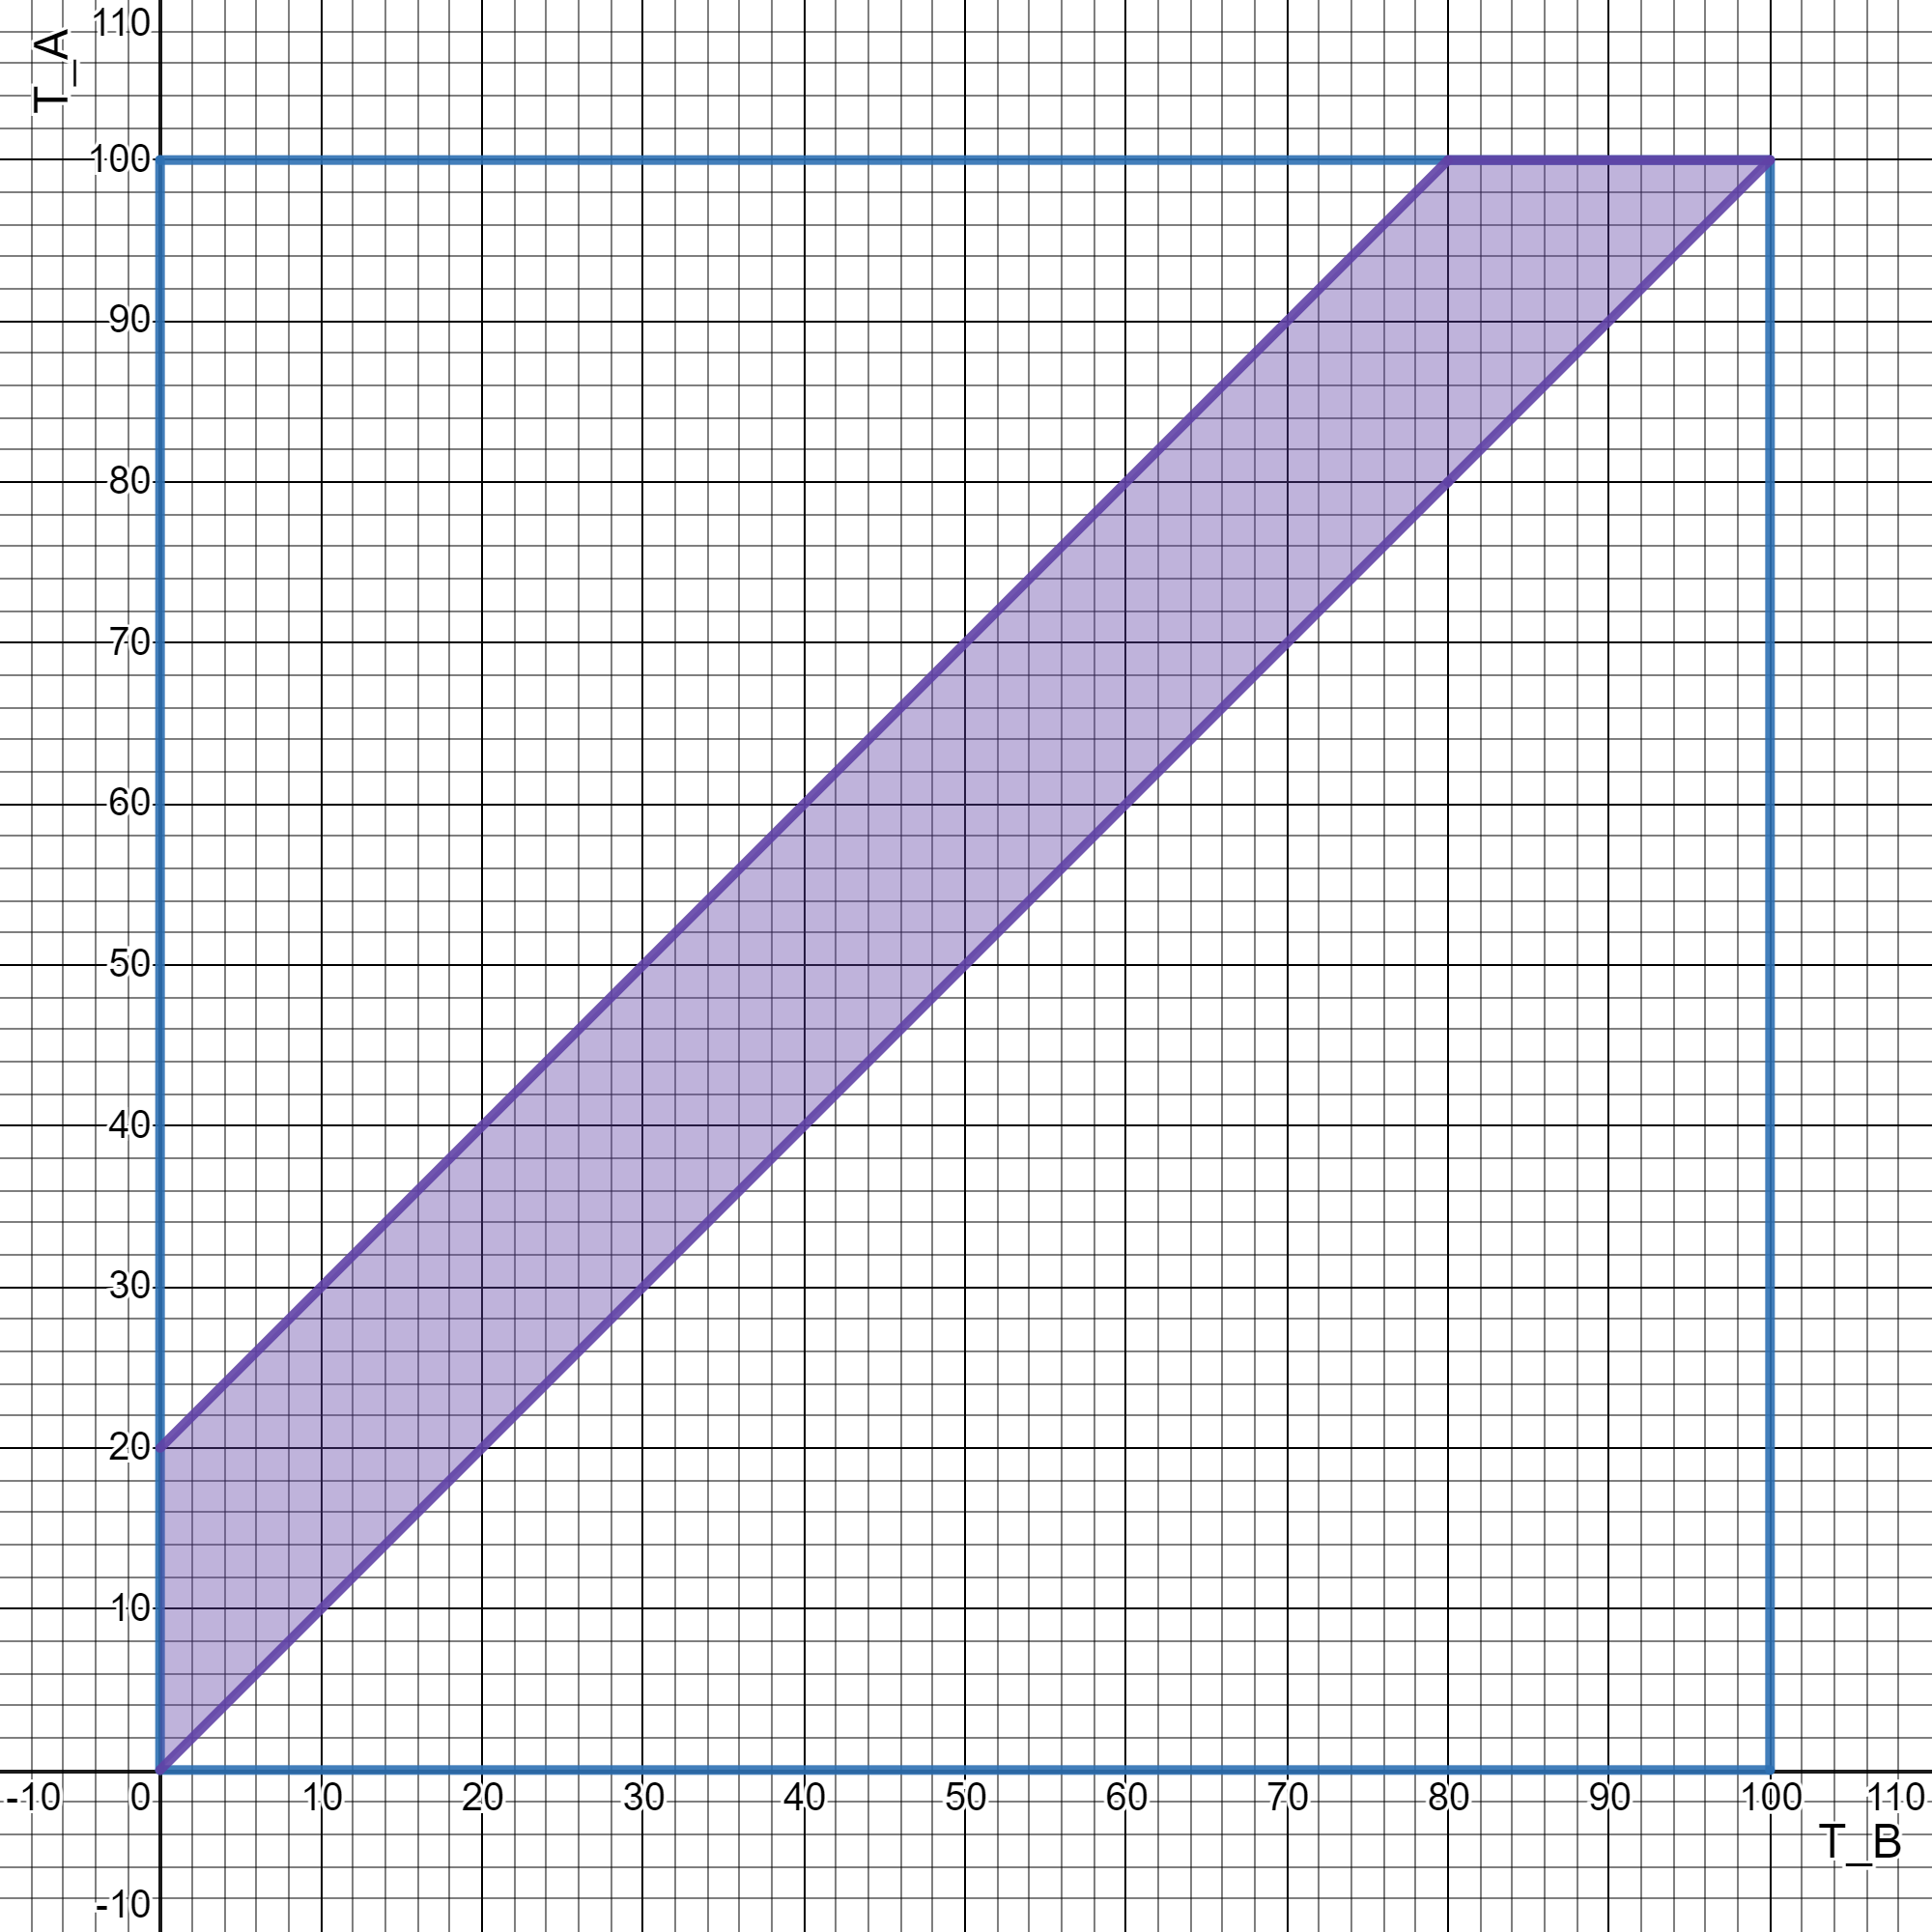
\includegraphics[width=.4\textwidth]{img/q2-c.png}
  \caption{}
\end{figure}

\begin{multicols}{2}
\begin{itemize}
  \item $\textnormal{The area of purple part} = 1800$
  \item $\textnormal{The area of the whole part} = 10^4$
\end{itemize}
\end{multicols}

So, the ratio of the purple area to whole area is the answer and it is $\dfrac{18}{100} = 0.18$.

\newpage
\subsection*{d)}

Again, if we think like the way mentioned in the hint. We are asked the ratio of the purple area to all area $\left[ 100 \times 100 \right]$ calculate the probability of the area of the Figure 2. The area is the following
\begin{equation*}
  \prob{(|T_A - T_B| \leq 30)}
\end{equation*}

\begin{figure}[ht!]
  \centering
  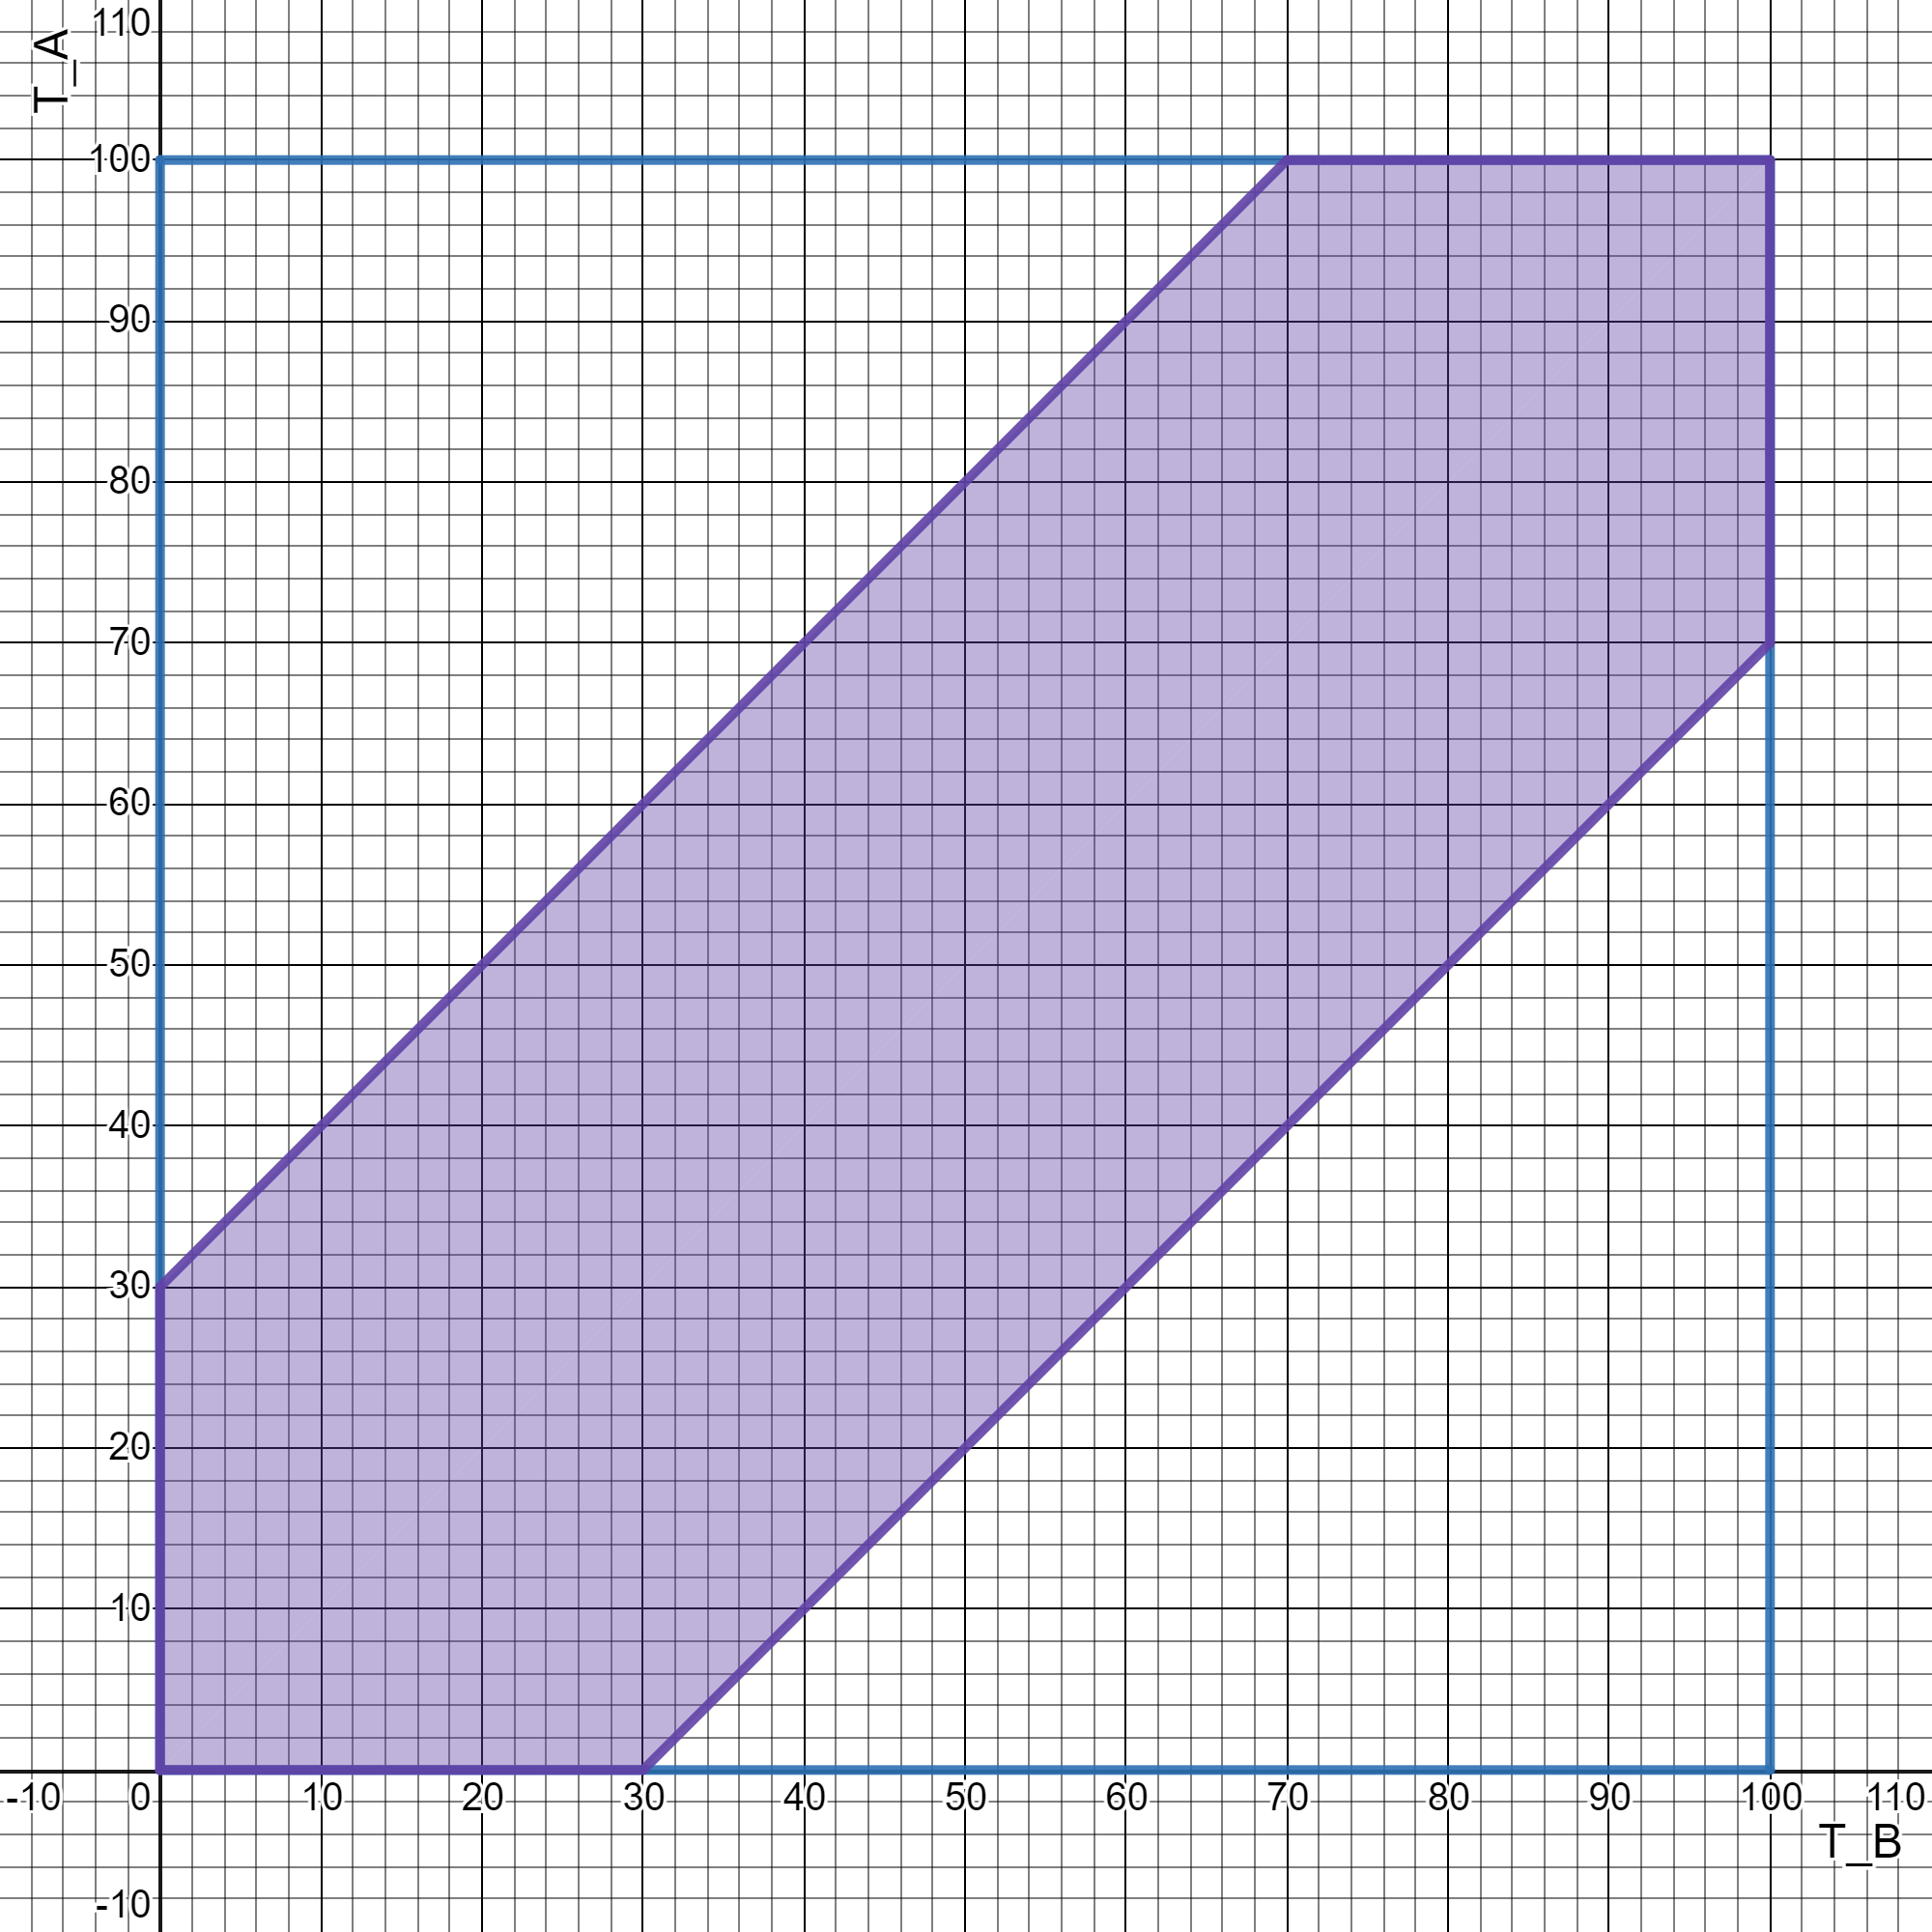
\includegraphics[width=.5\textwidth]{img/q2-d.png}
  \caption{}
\end{figure}

\begin{multicols}{2}
  \begin{itemize}
    \item $\textnormal{The area of purple part} = 5100$
    \item $\textnormal{The area of the whole part} = 10^4$
  \end{itemize}
\end{multicols}

So, the ratio of the purple area to whole area is the answer and it is $\dfrac{51}{100} = 0.51$.


\newpage
\section*{Answer 3}

\subsection*{a)}

% Let Xn = Exponential(λn) for 1 ≤ n ≤ N be independent random variables and T = min(X1, X2, . . . , XN ).
% What is the cdf of T?

For a random variable $X_i$, it has cdf
\begin{align*}
    F_{X_i} (x) &= \prob{X_i \leq x} = 1 - e^{-\lambda_i x_i} &x > 0
\end{align*}
for $i = 1, 2, ..., N$. Also, $T = \min(X_1, X_2, ..., X_N)$. Then the CDF of $T$ is
\begin{align*}
    F_T(t) &= \prob{T \leq t}\\
    &= 1 - \prob{T \geq t}\\
    &= 1 - \prob{\min(X_1, X_2, ..., X_N) \geq t}\\
    &= 1 - \prob{X_1 \geq t, X_2 \geq t, ..., X_N \geq t}\\
    &= 1 - \prob{X_1 \geq t} \prob{X_2 \geq t} \cdots \prob{X_N \geq t}\\
    &= 1 - e^{\lambda_1 t} e^{\lambda_2 t} \cdots e^{\lambda_N t}\\
    &= 1 - e^{-\sum_{i = 1}^{N} \lambda_i t}\ \ \ \ \ \ t > 0
\end{align*}

The answer is
\begin{equation*}
    F_T(t) = 1 - e^{-(\lambda_1 + \cdots + \lambda_N)t}
\end{equation*}


% Since given random variables are independent, one can notice that $T$ is also exponentially distributed, with parameter 
% \begin{equation*}
%     \lambda = \lambda_1 + \cdots + \lambda_N
% \end{equation*} 

% So, the pdf of $T$

% Distribution of $T$ is
% \begin{equation*}
%     \textnormal{Exponential}(\lambda_1 + ... + \lambda_N)
% \end{equation*}

% Then,

% \begin{equation*}
%     f(x) = \lambda e^{-\lambda x} = (\lambda_1 + ... + \lambda_N) e^{-(\lambda_1 + ... + \lambda_N)x}
% \end{equation*}

% So,

% \begin{align*}
%     \prob{T > x} = F(x) &= \int_{0}^{x} f(t) dt\\
%     &= \int_{0}^{x} (\lambda_1 + ... + \lambda_N) e^{-(\lambda_1 + ... + \lambda_N)t} dt\\
%     &= e^{-(\lambda_1 + ... + \lambda_N)t} \Big|_0^x\\
%     &= 1 - e^{-(\lambda_1 + ... + \lambda_N)x}
% \end{align*}


\subsection*{b)}

% We are given 10 different computers C1, C2, . . . , C10 the lifetimes of which are exponential random variables with means 10/n years (1 ≤ n ≤ 10), respectively. Each computer’s lifetime is independent from the others. What is the expected time before one of the computers fails?

% Let $t$ be the fail of one computer. We need to acquire a formula to calculate

% Let $X_n = \textnormal{Exponential}(\lambda_n)$ for $1 \leq n \leq N$ be independent random variables. The probability that $X_i$ is the minimum can be obtained by conditioning:

% \begin{align*}
%     \prob{X_i \textnormal{ is the minimum}} &= \prob{X_i < X_j \textnormal{ for } j \neq i}\\
%     &= \int_{0}^{\infty} \prob{X_i < X_j \textnormal{ for } j \neq i\ |\ X_i = t} \lambda_i e^{-\lambda_i t} dt\\
%     &= \prob{t < X_j \textnormal{ for } j \neq i} \lambda_i e^{-\lambda_i t} dt\\
%     &= \int_{0}^{\infty} \lambda_i e^{-\lambda_i t} \prod_{j \neq i}^{} \prob{X_j > t} dt\\
%     &= \int_{0}^{\infty} \lambda_i e^{-\lambda_i t} \prod_{j \neq i}^{} e^{-\lambda_j t} dt\\
%     &= \lambda_i \int_{0}^{\infty} e^{-(\lambda_1 + ... + \lambda_N)t} dt\\
%     &= \lambda_i \frac{- e^{-(\lambda_1 + \cdots + \lambda_N)t}}{\lambda_1 + \cdots + \lambda_N} \Biggl|_0^{\infty}\\
%     &= \frac{\lambda_i}{\lambda_1 + \cdots + \lambda_N}
% \end{align*}

% \begin{equation*}
%     \expc{X} = \dfrac{1}{10 + 5 + \dfrac{10}{3} + \dfrac{10}{4} + 2 + \dfrac{10}{6} + \dfrac{10}{7} + \dfrac{10}{8} + \dfrac{10}{9} + 1} = \dfrac{252}{7381}
% \end{equation*}

From question, there are 10 $\expc{X_i}$'s:
\begin{multicols}{4}
\begin{itemize}
    \item $\expc{X_1} = \dfrac{10}{1}$
    \item $\expc{X_2} = \dfrac{10}{2}$
    \item $\expc{X_3} = \dfrac{10}{3}$
    \item $\expc{X_4} = \dfrac{10}{4}$
    \item $\expc{X_5} = \dfrac{10}{5}$
    \item $\expc{X_6} = \dfrac{10}{6}$
    \item $\expc{X_7} = \dfrac{10}{7}$
    \item $\expc{X_8} = \dfrac{10}{8}$
    \item $\expc{X_9} = \dfrac{10}{9}$
    \item $\expc{X_{10}} = \dfrac{10}{10}$
\end{itemize}
\end{multicols}

Since $\lambda_i = \dfrac{1}{\expc{X_i}}$, from question, there are 10 $\lambda$'s:
\begin{multicols}{5}
\begin{itemize}
    \item $\lambda_1 = \dfrac{1}{10}$
    \item $\lambda_2 = \dfrac{2}{10}$
    \item $\lambda_3 = \dfrac{3}{10}$
    \item $\lambda_4 = \dfrac{4}{10}$
    \item $\lambda_5 = \dfrac{5}{10}$
    \item $\lambda_6 = \dfrac{6}{10}$
    \item $\lambda_7 = \dfrac{7}{10}$
    \item $\lambda_8 = \dfrac{8}{10}$
    \item $\lambda_9 = \dfrac{9}{10}$
    \item $\lambda_{10} = \dfrac{10}{10}$
\end{itemize}
\end{multicols}

We found the CDF in part a. By using that CDF, we can calculate $\expc{X}$ and we reach
\begin{equation*}
    \expc{X} = \frac{1}{\lambda_1 + \cdots + \lambda_N}
\end{equation*}

So, when we use $\expc{X}$ for 10 variables in question

\begin{equation*}
    \expc{X} = \dfrac{1}{\dfrac{1}{10} + \dfrac{2}{10} + \dfrac{3}{10} + \dfrac{4}{10} + \dfrac{5}{10} + \dfrac{6}{10} + \dfrac{7}{10} + \dfrac{8}{10} + \dfrac{9}{10} + \dfrac{10}{10}} = \dfrac{2}{11}
\end{equation*}


\section*{Answer 4}

% Central Limit Theorem applies to all these distributions with sufficiently large $n$ in the case of Binomial, k for Negative Binomial, and α for Gamma variables.


% According to Central Limit Theorem, as long as $n$ is large, one can use Normal distribution to compute probabilities about $S_n$. So, in here $n = 30.000$, then we can use 

%%%%%%%%%%%%%%%%%%%%%%%%%%%%%%%%%%%%%%%%%%


%variables are Binomial; in other words, they are Binomial distribution. For small 

% Also, the Central Limit Theorem is applicable to Binomial variables with sufficiently large $n$. So, we can use the Binomial($n, p$). since p is not small or large enough. Instead, $0.05 \leq p \leq 0.95$; therefore, we can 

%%%%%%%%%%%%%%%%%%%%%%%%%%%%%%%%%%%%%%%%%%

% In here, let 
% \begin{itemize}
%   \item $X_1 = 70$ people from undergraduate
%   \item $X_2 = 71$ people from undergraduate
%   \item[] $\cdot$
%   \item[] $\cdot$
%   \item[] $\cdot$
%   \item $X_{31} = 100$ people from undergraduate   
% \end{itemize}
% We need to find the sum of the probability of each one. So, the Central Limit Theorem is applicable to Binomial variables with sufficiently large $n$. 
% So, $S_n = X_1 + \cdots + X_{31}$. For small $p$, we can use Poisson, but out $p$is not small. In such situation, $0.05 \leq p \leq 0.95$, we can use the following
% \begin{equation*}
%   \textnormal{Binomial}(n, p) \approx Normal \left( \mu = np, \sigma = \sqrt{np(1-p)} \right)
% \end{equation*}

%%%%%%%%%%%%%%%%%%%%%%%%%%%%%%%%%%%%%%%5

According to Central Limit Theorem, if $n$ is sufficiently large and $p$ satisfies the condition $0.05 \leq p \leq 0.95$, then all distribution can be thought as Normal distribution. Since all variables are Binomial, we can use the following
\begin{equation*}
  \textnormal{Binomial}(n, p) \approx \textnormal{Normal}\left( \mu = np, \sigma = \sqrt{np(1-p)} \right)
\end{equation*}

\subsection*{a)}

We need to determine $n$, $p$ and, by using these, we need to find $\mu$, $\sigma$

\begin{multicols}{2}
  \begin{itemize}
    \item $n = 100$
    \item $p = 0.74$
    \item $\mu = np = 74$
    \item $\sigma = \sqrt{np(1-p)} \approx 4.39$
  \end{itemize}
\end{multicols}

And we are asked the following, ($X$ = the number of undergraduate students in the group.)

\begin{align*}
  \prob{X \geq 70} &= \prob{X \geq 69.5} &(\textit{Continuity correction})\\
  &= 1 - \prob{X \leq 69.5}\\
  &= 1 - \prob{\dfrac{X - \mu}{\sigma} \leq \dfrac{69.5 - \mu}{\sigma}}\\
  &= 1 - \prob{\dfrac{X - 74}{4.38634244} \leq \dfrac{69.5 - 74}{4.38634244}}\\
  &= 1 - \prob{Z \leq \dfrac{69.5 - 74}{4.38634244}}\\
  &= 1 - \prob{Z \leq - 1.025911693}\\
  &= 1 - \Phi(- 1.025911693)\\
  &= 1 - 0.1525 = 0.8475 \approx 0.85
\end{align*}

\newpage
\subsection*{b)}

We need to determine $n$, $p$ and, by using these, we need to find $\mu$, $\sigma$

\begin{multicols}{2}
  \begin{itemize}
    \item $n = 100$
    \item $p = 0.10$
    \item $\mu = np = 10$
    \item $\sigma = \sqrt{np(1-p)} = 3$
  \end{itemize}
\end{multicols}

And we are asked the following, ($X$ = the number of people pursuing a doctoral degree in the group.)

\begin{align*}
  \prob{X \leq 5} &= \prob{X \leq 5.5} &(\textit{Continuity correction})\\  
  &= \prob{\dfrac{X - \mu}{\sigma} \leq \dfrac{5.5 - \mu}{\sigma}}\\
  &= \prob{\dfrac{X - 10}{3} \leq \dfrac{5.5 - 10}{3}}\\
  &= \prob{Z \leq - 1.50}\\
  &= \Phi(- 1.50)\\
  &= 0.066807 \approx 0.07
\end{align*}



% \begin{align*}
%   \prob{0 \leq X \leq 5} &= \prob{\dfrac{0 - \mu}{\sigma} \leq \dfrac{X - \mu}{\sigma} \leq \dfrac{5 - \mu}{\sigma}}\\
%   &= \prob{\dfrac{0 - 10}{3} \leq \dfrac{X - 10}{3} \leq \dfrac{5 - 10}{3}}\\
%   &= \prob{- 3.33 \leq Z \leq - 1.67}\\
%   &= \Phi(- 1.67) - \Phi(- 3.33)\\
%   &= 0.0475 - 0.0004 = 0.0471
% \end{align*}


\end{document}

